%%%%% Document Setup %%%%%%%%

\documentclass[10pt, twocolumn]{revtex4}    % Font size (10,11 or 12pt) and column number (one or two).

\usepackage{times}                          % Times New Roman font type

\usepackage[a4paper, left=1.85cm, right=1.85cm,
 top=1.85cm, bottom=1.85cm]{geometry}       % Defines paper size and margin length

\usepackage[font=small,
labelfont=bf]{caption}                      % Defines caption font size as 9pt and caption title bolded

\usepackage{mathtools,amssymb}
\usepackage{graphics,graphicx,epsfig,ulem}	% Makes sure all graphics works
\usepackage{amsmath} 						% Adds mathematical features for equations
%\usepackage{siunitx}
\usepackage{textcomp}
\usepackage{enumitem}
\usepackage{bm}
\usepackage{lipsum}
\usepackage[toc,page]{appendix}
\usepackage{booktabs}
\usepackage{rotating}
\usepackage{siunitx}
\usepackage{multirow}
\usepackage{ulem}
\usepackage{array}
\newcolumntype{L}[1]{>{\raggedright\arraybackslash}p{#1}}

\usepackage{etoolbox}                       % Customise date to preferred format
\makeatletter
\patchcmd{\frontmatter@RRAP@format}{(}{}{}{}
\patchcmd{\frontmatter@RRAP@format}{)}{}{}{}
\renewcommand\Dated@name{}
\newcommand{\rom}[1]{\uppercase\expandafter{\romannumeral #1\relax}}
\makeatother

%\usepackage[flushleft]{threeparttable}

\usepackage{fancyhdr}

\pagestyle{fancy}                           % Insert header
\renewcommand{\headrulewidth}{0pt}
\lhead{P. Einarsson Nielsen}                          % Your name
\rhead{TITLE}           % Your report title               

\def\bibsection{\section*{References}}        % Position refernce section correctly


\AtBeginDocument{
	\heavyrulewidth=.08em
	\lightrulewidth=.05em
	\cmidrulewidth=.03em
	\belowrulesep=.65ex
	\belowbottomsep=0pt
	\aboverulesep=.4ex
	\abovetopsep=0pt
	\cmidrulesep=\doublerulesep
	\cmidrulekern=.5em
	\defaultaddspace=.5em
}
\renewcommand{\arraystretch}{1.2}


%%%%% Document %%%%%
\begin{document}                     


\title{TITLE} 
\date{Submitted: \today{}}
\author{P. Einarsson Nielsen}
\affiliation{\normalfont Affiliation}

\begin{abstract}
	\lipsum[1]

\end{abstract}

\maketitle
\thispagestyle{plain} % produces page number for front page



\section{Introduction} \label{s:intro}

\begin{itemize}
	\item Detail balance
	\item Ergodic
	\item Stochastic
	\item Entropy driven phase transitions
	\item Equations of state
	
\end{itemize}

%\lipsum[1-8]

%\subsection{Subsection} \label{ss}
%\lipsum[1-3]


\section{Methodology} \label{s:methods}
A system of $N=1000$ particles interacting with the Lennard-Jones potential was simulated using the Metropolis Monte Carlo algorithm (hereafter referred to as MC). The particles were initialised in a face-centred cubic (FCC) lattice within a squared container of volume $V$. Conventional boundary conditions, where a particle which moves beyond the boundary of its container is moved to the opposite side, were applied. MC involves applying a random Cartesian move to each particle in turn, described by
\begin{displaymath}
\Delta{}\bar{s} = d\left(\bar{\xi}-0.5\right)
\end{displaymath}
where $\bar{s}$ and $\bar{\xi}$ are three-vectors containing the move and random numbers between 0 and 1 respectively and $d$ is the maximum displacement.
A move was accepted if it resulted in a decrease in the total potential energy of the system. If not, the move was accepted with a probability proportional to the Boltzmann factor of the resulting state,
\begin{displaymath}
\exp{\frac{\Delta{}U}{k_\text{B}T}}.
\end{displaymath}
where $\Delta{}U, k_\text{B}, T$ are the change in potential energy, Boltzmann constant and system temperature respectively.
This over-weights rarer configurations and is known as importance sampling. At equilibrium, each move is reversible by a move in the opposite direction and, as such, this algorithm satisfies detail balance.
The system was equilibrated over $10^7$ moves such that the initial FCC structure is not present. The maximum displacement, $d$ is adjusted periodically during this equilibration such that the 30-50\% of moves were accepted.
The system was then evolved over another $10^7$ moves and its configuration sampled every $10^3$ moves. The radial distribution function, $g(r)$, was then calculated and averaged over each particle. The radial distribution function tells us the probability, relative to the ideal gas case, of finding a molecule at a given distance from a reference particle and can be expressed as
\begin{displaymath}
g(r) = \frac{n(r)}{n_\text{ideal}(r)}
\end{displaymath}
where $n_\text{ideal} = \rho{}4\pi{}r^{2}\Delta{}r$, $n(r)$ is the number of particles within a shell of thickness $\Delta{}r$ at a distance $r$, $\rho{}$ is the number density of the system.

System properties relating to its configuration can be computed from $g(r)$. We compute the excess internal energy per particle by the energy equation \ref{eq:energy} and the excess pressure of the system by the virial equation \ref{eq:pressure}.

\begin{equation}
u^{*} = 2\pi{}\rho{}\int_{0}^{r_\text{max}}U_\text{LJ}(r)g(r)r^{2}dr
\label{eq:energy}
\end{equation}

\begin{equation}
p^{*} = P - \rho{}k_\text{B}T = - \frac{2\pi}{3}\rho{}^{2} \int_{0}^{r_\text{max}}\frac{U_\text{LJ}(r)}{dr}g(r)r^{3}dr
\label{eq:pressure}
\end{equation}

The integrals in equations \ref{eq:energy} and \ref{eq:pressure} were approximated as sums where $dr \rightarrow{} \Delta{}r = 0.02\sigma{}$, calculated up to a maximum distance of $r_\text{max} = 6\sigma{}$. (JUSTIFY THIS)



\section{Model} \label{s:model}
Our simulated system consists of $N$ number of particles enclosed in a cubic container of volume $V$. The potential energy between any two particles in the system is given by the Lennard-Jones potential, expressed in the reduced unit scheme as
\begin{equation}
U_{LJ} = 4\left(\frac{1}{r^{12}}-\frac{1}{r^{6}}\right)
\end{equation}
where $r$ is the reduced distance between the particles.
The number of particles in the system was kept constant for every initial configuration and, as such, achieving a given reduced density required the container length to be varied. When applying perturbations to a particle in the system, the interaction potential was considered for every other particle in the system under periodic boundary conditions, or up to half the container length.

Virial equation and configuration energy per particle


The model and method were verified by direct comparison to Monte Carlo results at liquid and vapour-like densities along isotherms $T^{*}=0.85, 0.90$ published by United States' National Institute of Standard and Technology (NIST). NIST's results were for 500 particles whose Lennard-Jones interaction had been truncated to $3\sigma{}$ and standard long range corrections had been applied. Their systems were equilibrated for $5.0\text{e}7$ moves and quantities calculated over $2.5\text{e}8$ moves. Figure \ref{fig:NIST_comparison} shows the configuration energy per particle, $u^*$, and virial pressure, $p^{*} = P - \rho{}kT$ for both our system and NIST's. Our results were obtained as described in section \ref{s:methods}. See appendix \ref{a:NIST} for the values and their associated uncertainties of NIST's and our simulations.

\begin{figure}
	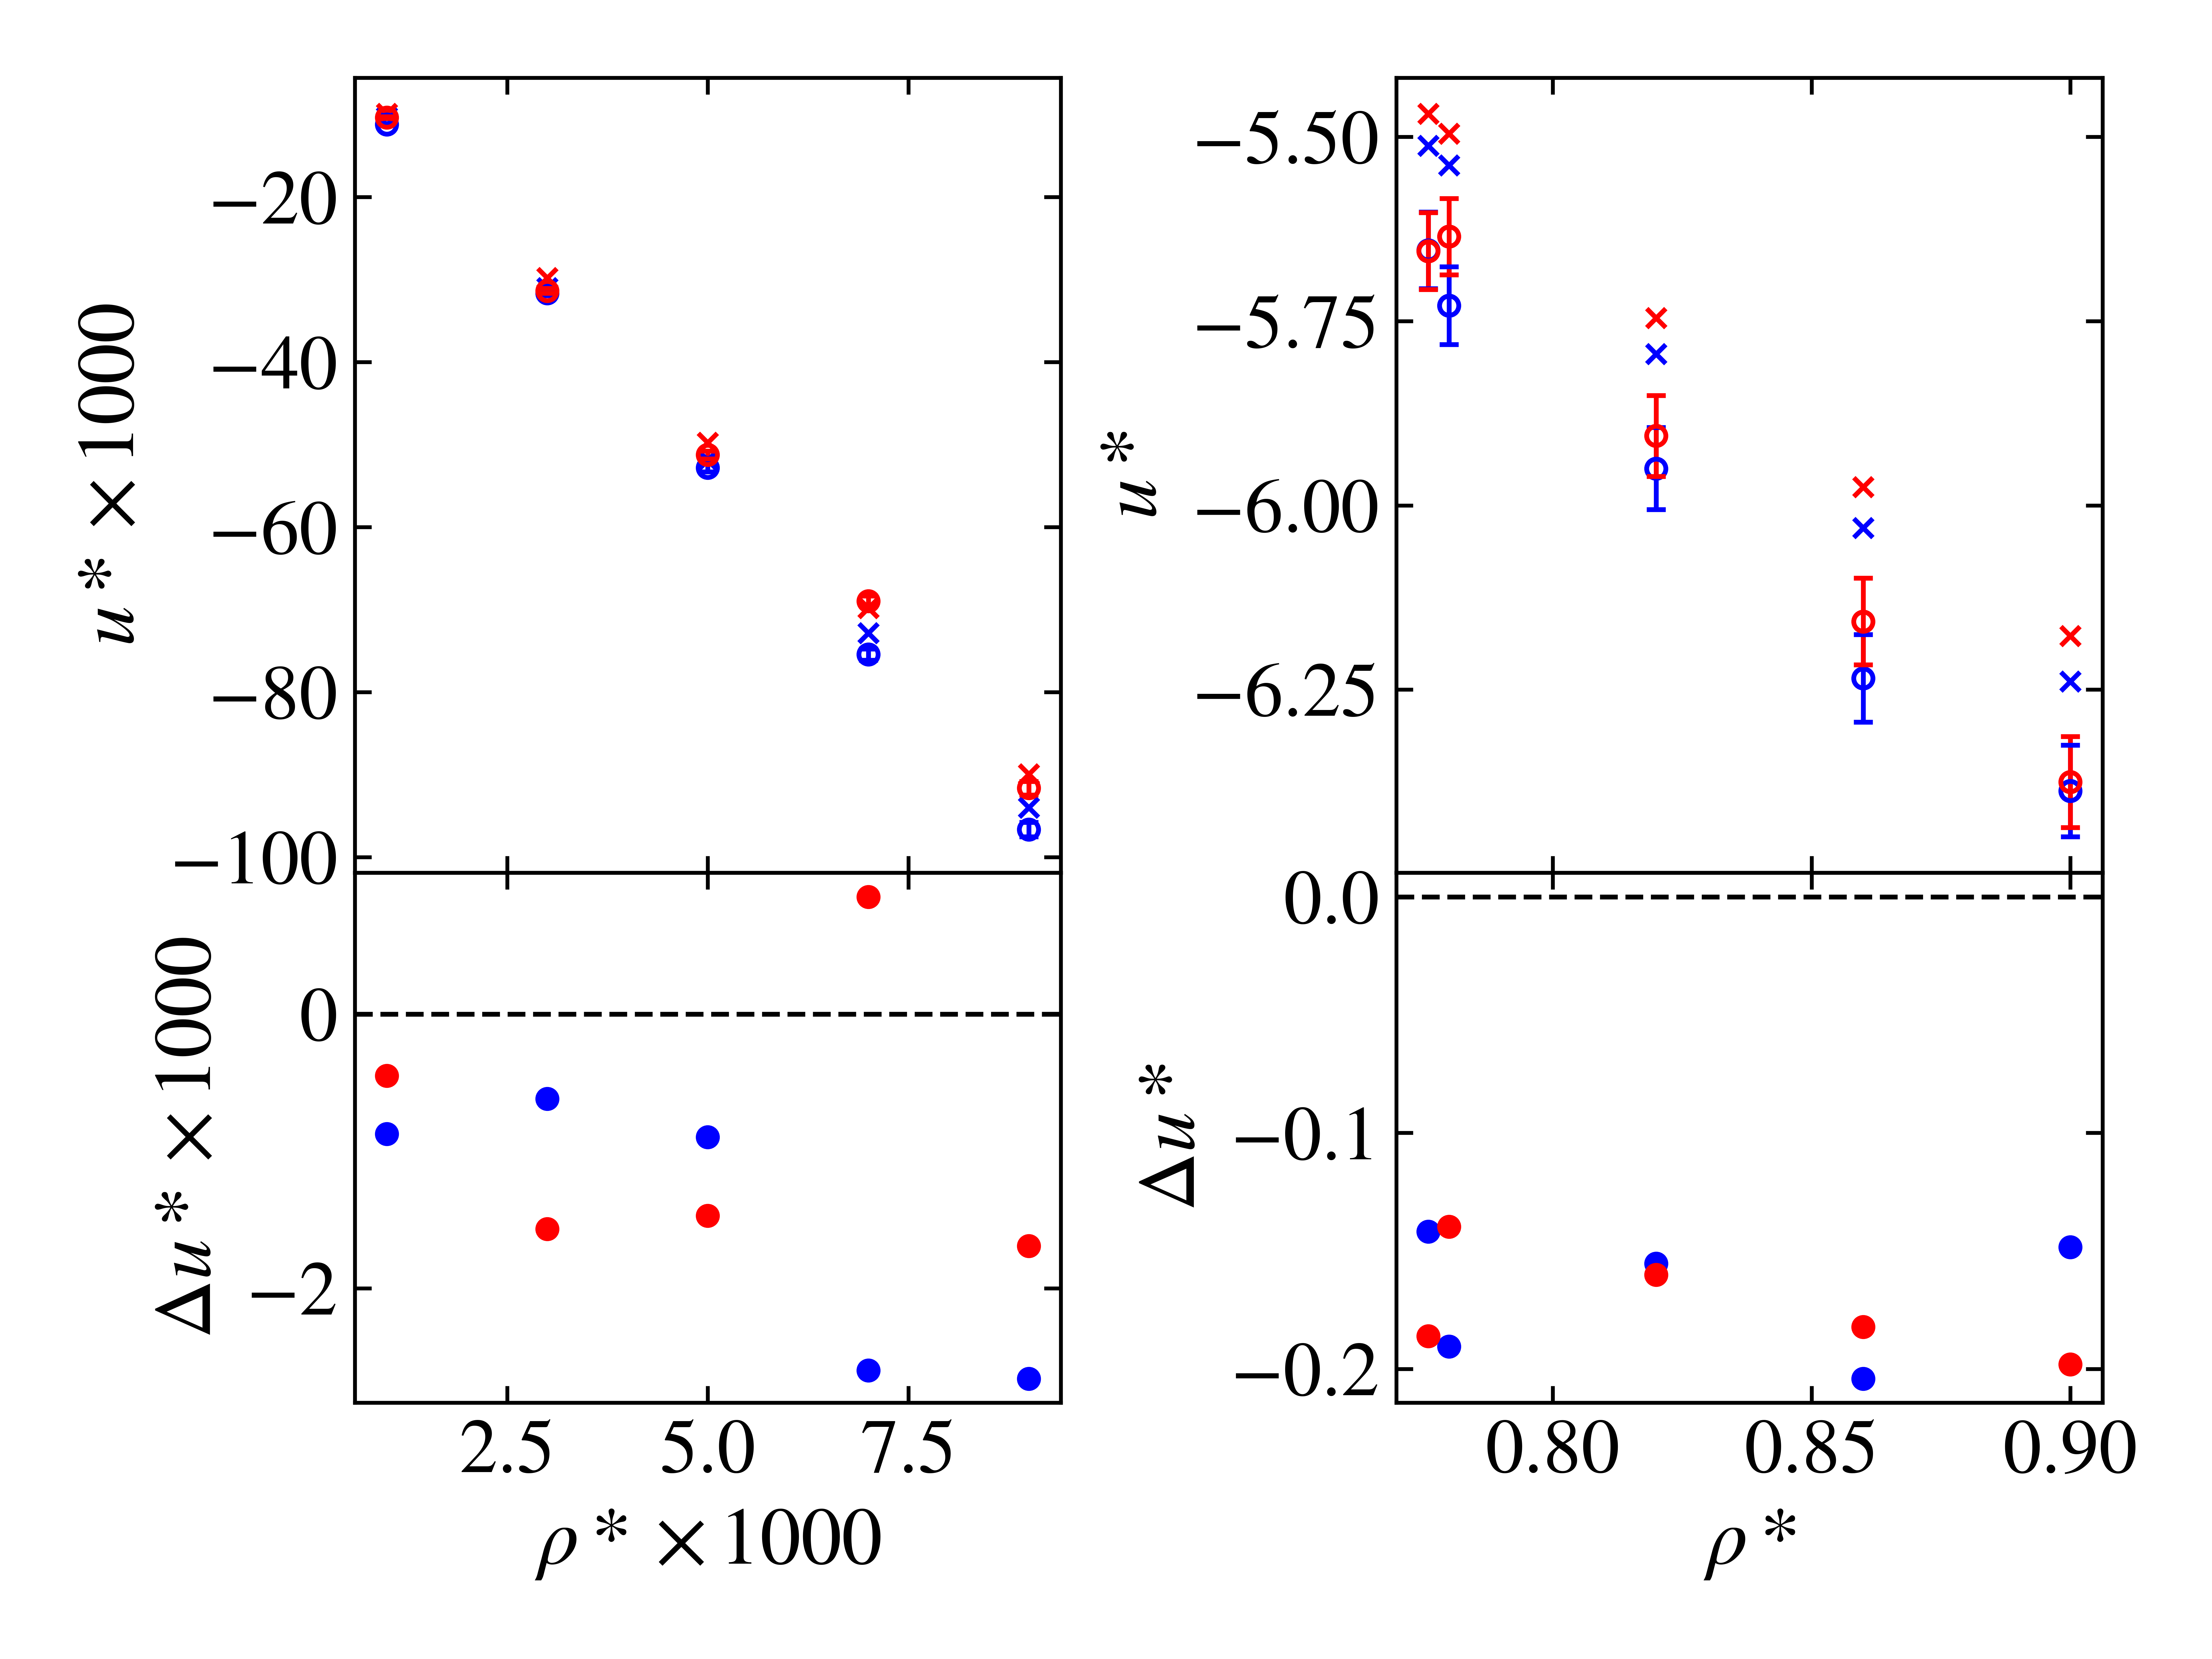
\includegraphics[width=\linewidth]{figures/NIST_comparison/NIST_u.png}
	\caption{Excess energy per particle, $u^{*}$, at vapour-like (upper-left panel, note that these values have been scaled by a factor of 1000) and liquid-like (upper-right panel) densities, $\rho{}^{*}$. Our MC results and those of the National Institute of Science and Technology (NIST) are represented by unfilled circles and crosses respectively. Data is shown for isotherms $T^{*}=0.85, 0.90$ by blue and red markers respectively. Error bars for our MC data show the standard error in the mean. Error bars are not shown for NIST's data for visual clarity. Residuals are shown in the lower panels. A dotted line has been added along the zero-residual for reference.}
	\label{fig:NIST_u}
\end{figure}

\begin{figure}
	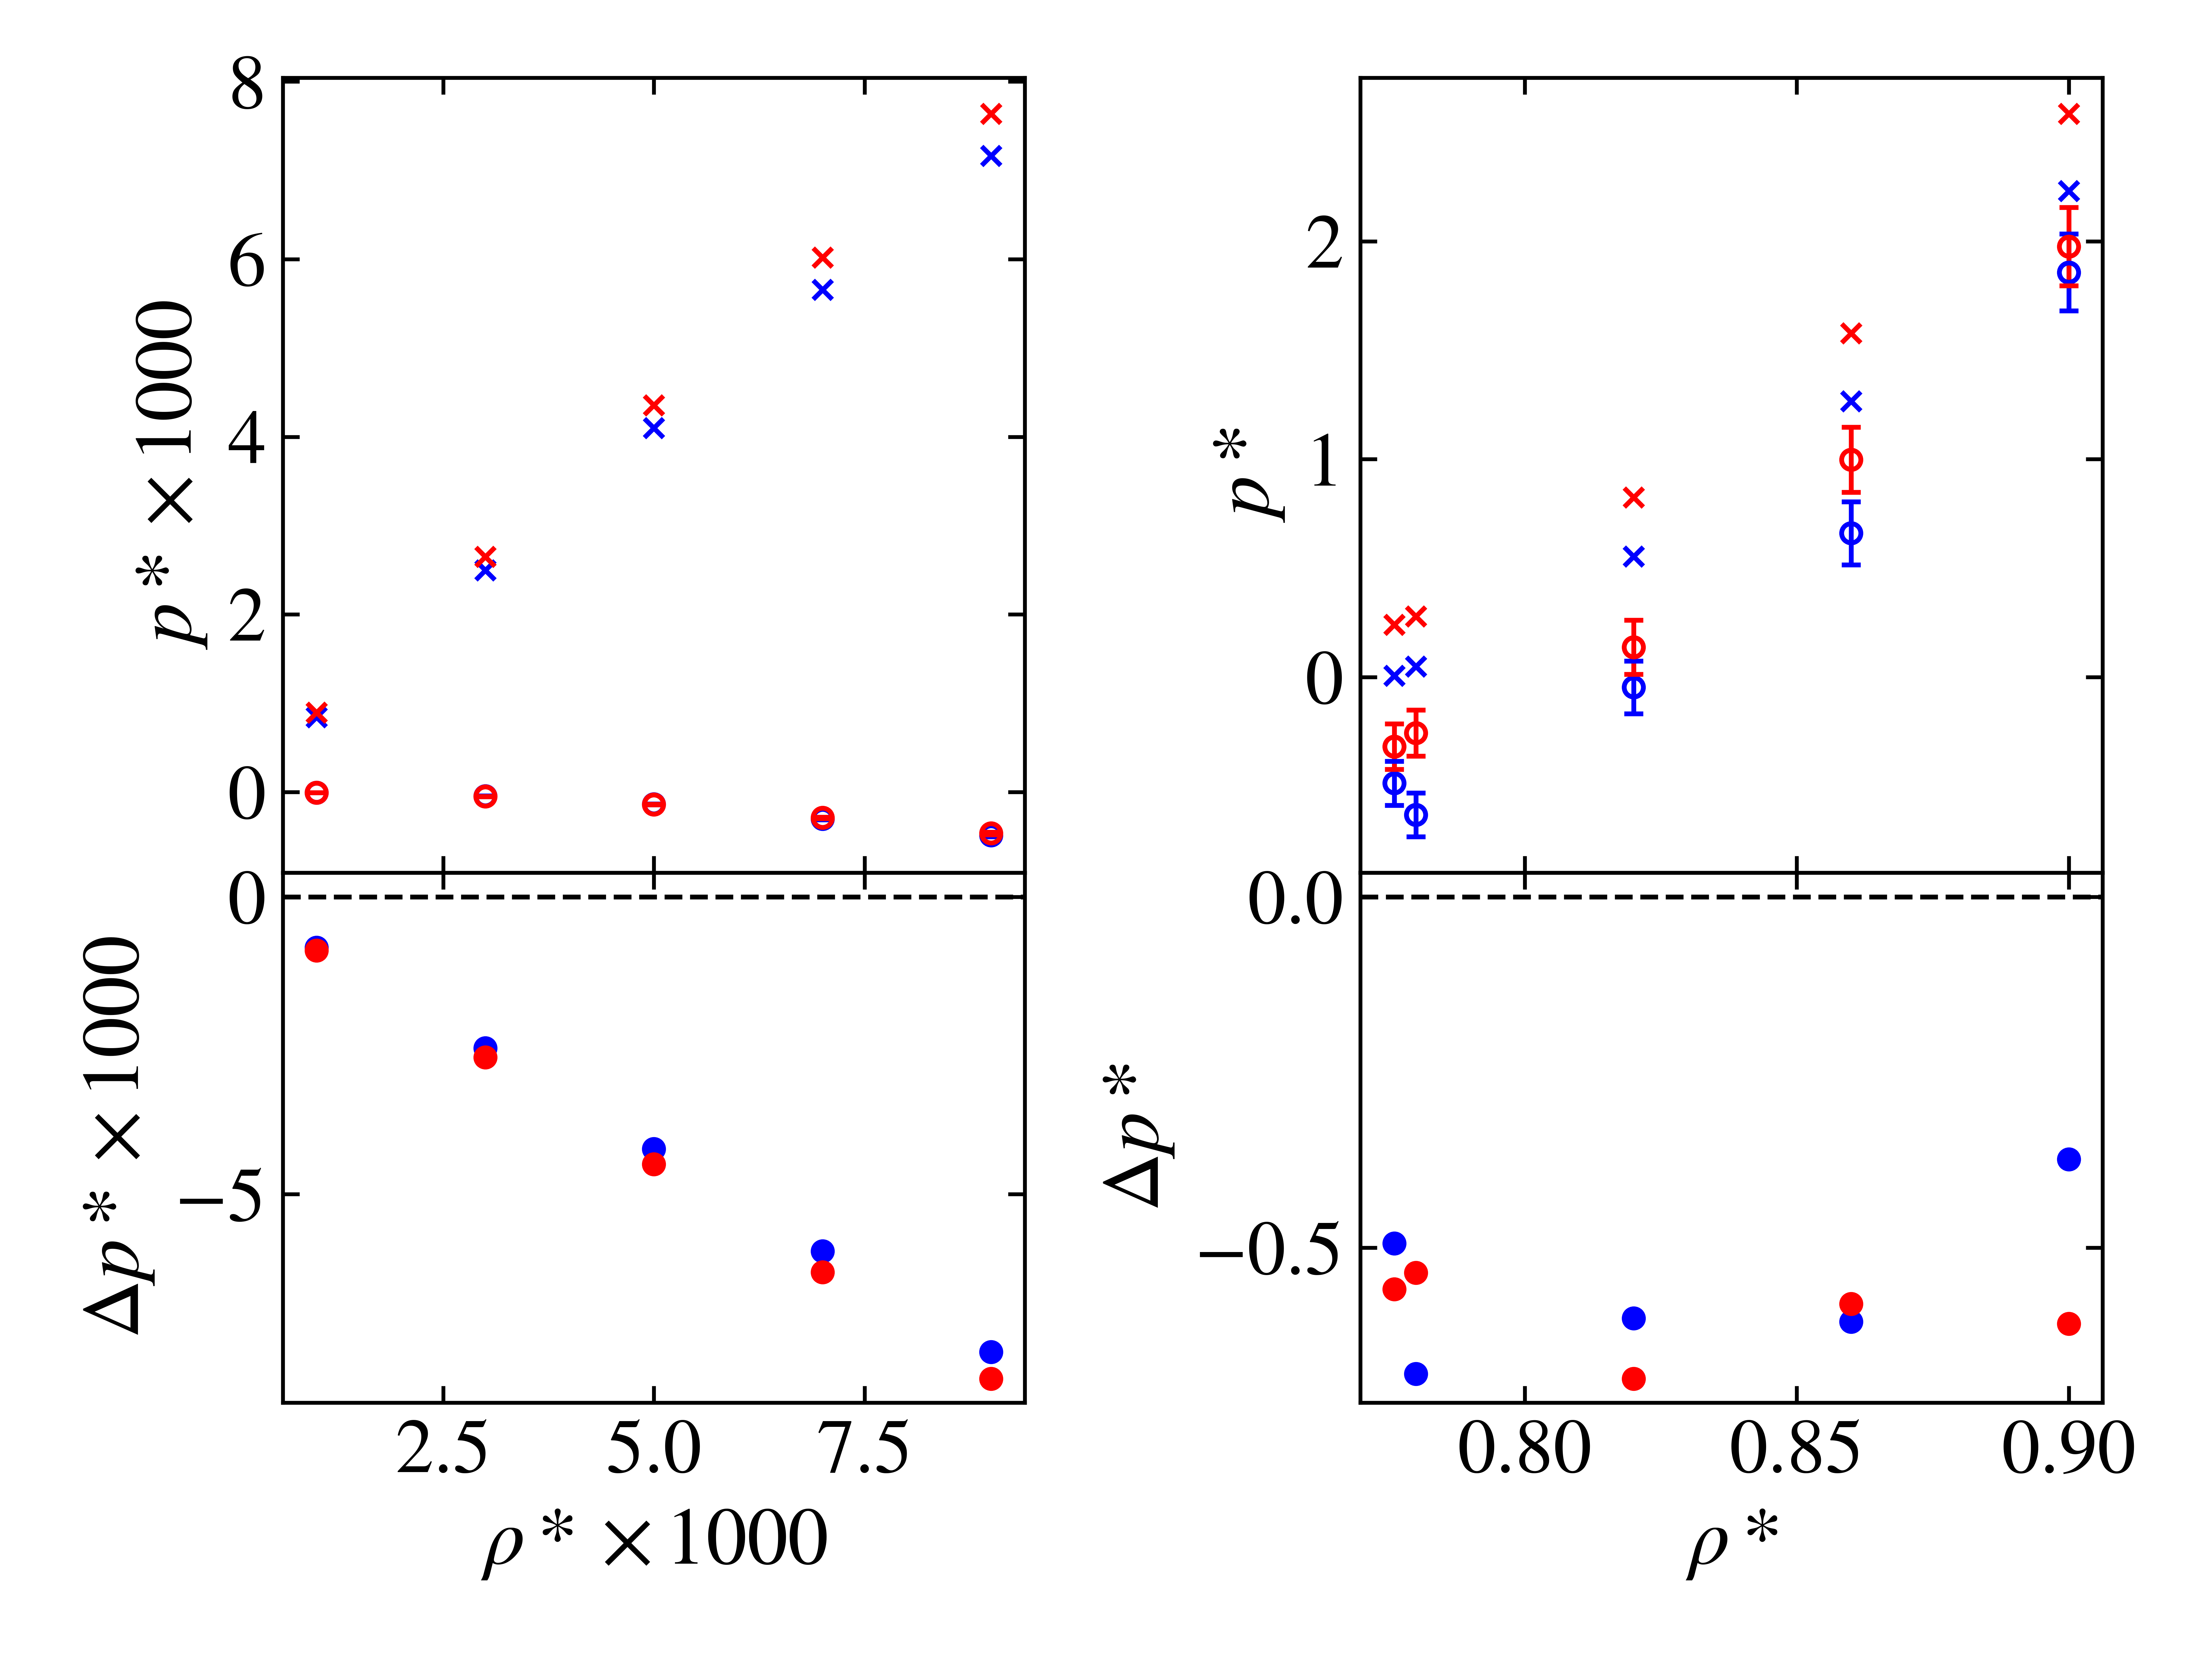
\includegraphics[width=\linewidth]{figures/NIST_comparison/NIST_p.png}
	\caption{Excess pressure, $p^{*}$, at vapour-like (upper-left panel, note that these values have been scaled by a factor of 1000) and liquid-like (upper-right panel) densities, $\rho{}^{*}$. Our MC results and those of the National Institute of Science and Technology (NIST) are represented by unfilled circles and crosses respectively. Data is shown for isotherms $T^{*}=0.85, 0.90$ by blue and red markers respectively. Error bars for our MC data show the standard error in the mean. Error bars are not shown for NIST's data for visual clarity. Residuals are shown in the lower panels. A dotted line has been added along the zero-residual for reference.}
	\label{fig:NIST_p}
\end{figure}



\section{Results} \label{s:results}
%\lipsum[1-10]

The resulting excess energy per particle and excess pressure as functions of the reduced density are shown in figures \ref{fig:excessEnergy} and \ref{fig:excessPressure} respectively. Configuration energy can be seen to reduce from approximately $0$ at $\rho{}^*=0$ before reaching some local minimum value and increasing. The value of $\rho{}^*$ at which this local minima is reached appears to vary as a function of the system temperature; the absolute value of the minima is decreased and occurs at smaller $\rho{}^*$ at higher temperatures when compared to that of lower temperatures.

Interpretation - at lower densities we are essentially considering an ideal gas; compare to total energy u-config + u-kinetic

\begin{figure}
	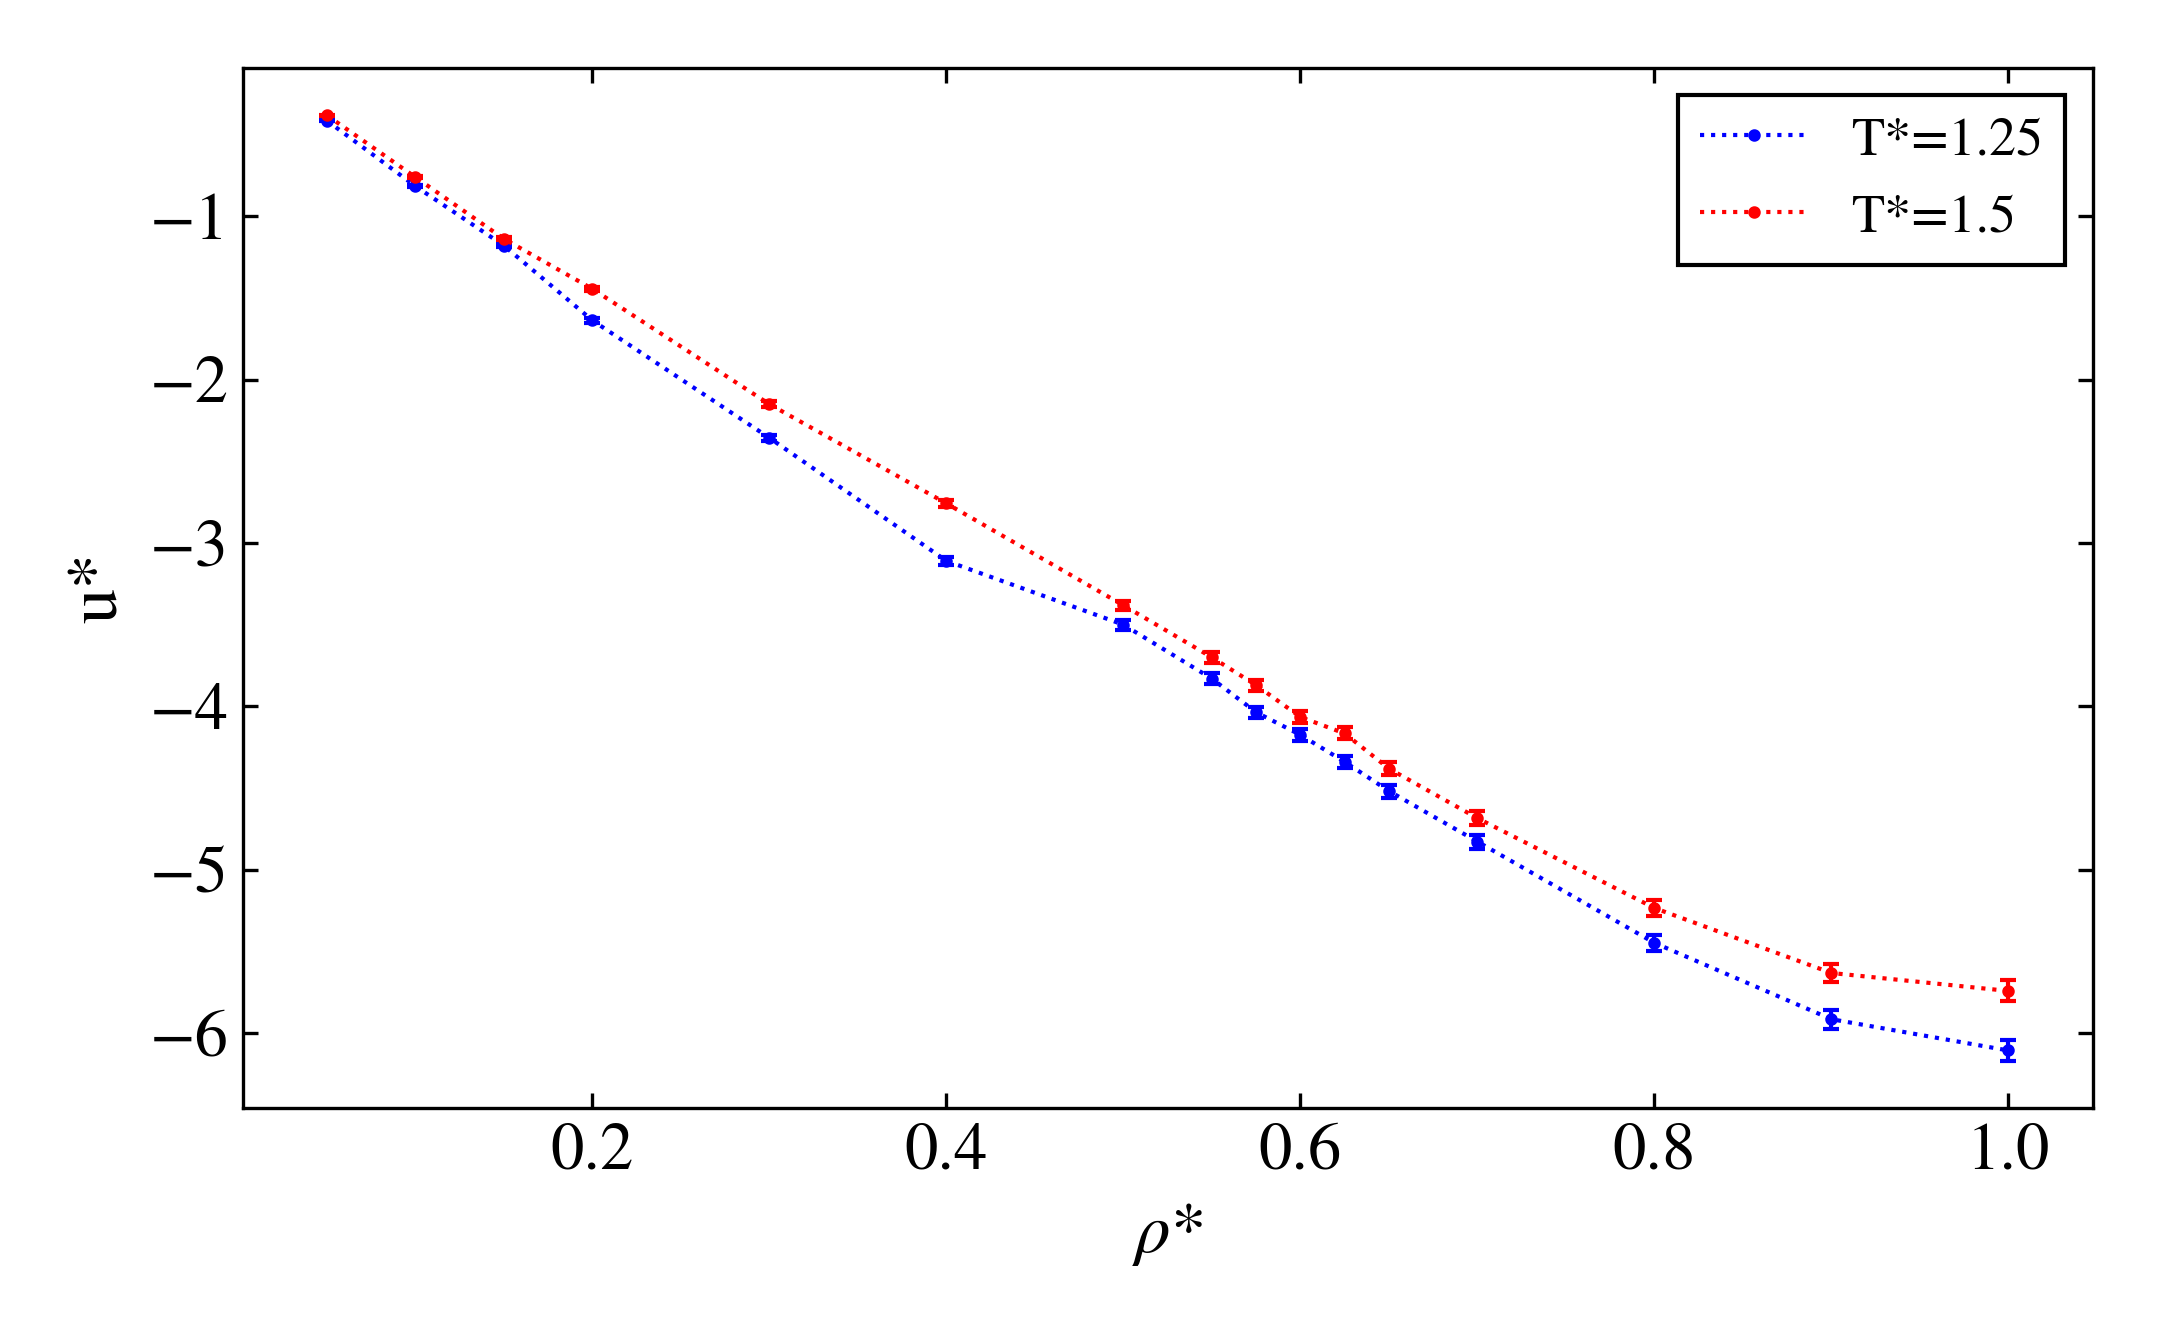
\includegraphics[width=\linewidth]{figures/excessEnergyPressure/excessEnergy.png}
	\caption{MC results for the excess energy per particle, $u^{*}$, against density, $\rho{}^{*}$ along four isotherms $T^{*}=0.75, 1.00, 1.25, 1.50$, each represented by a colour ranging from blue to red. Error bars show the standard error in the mean. Dotted lines have been added to guide the eye.}
	\label{fig:excessEnergy}
\end{figure}

Reduced pressure can be seen to increase *exponentially* from approximately $0$ at $\rho{}^*=0$ with increasing $\rho{}^*$. The rate of increase can be seen to be greater at higher than lower temperatures.


At very low $\rho{}^*$ the system temperature is observed to have little impact on the configuration energy or pressure. However at larger $\rho{}^*$ the difference between systems of different temperatures increases.


\begin{figure}
	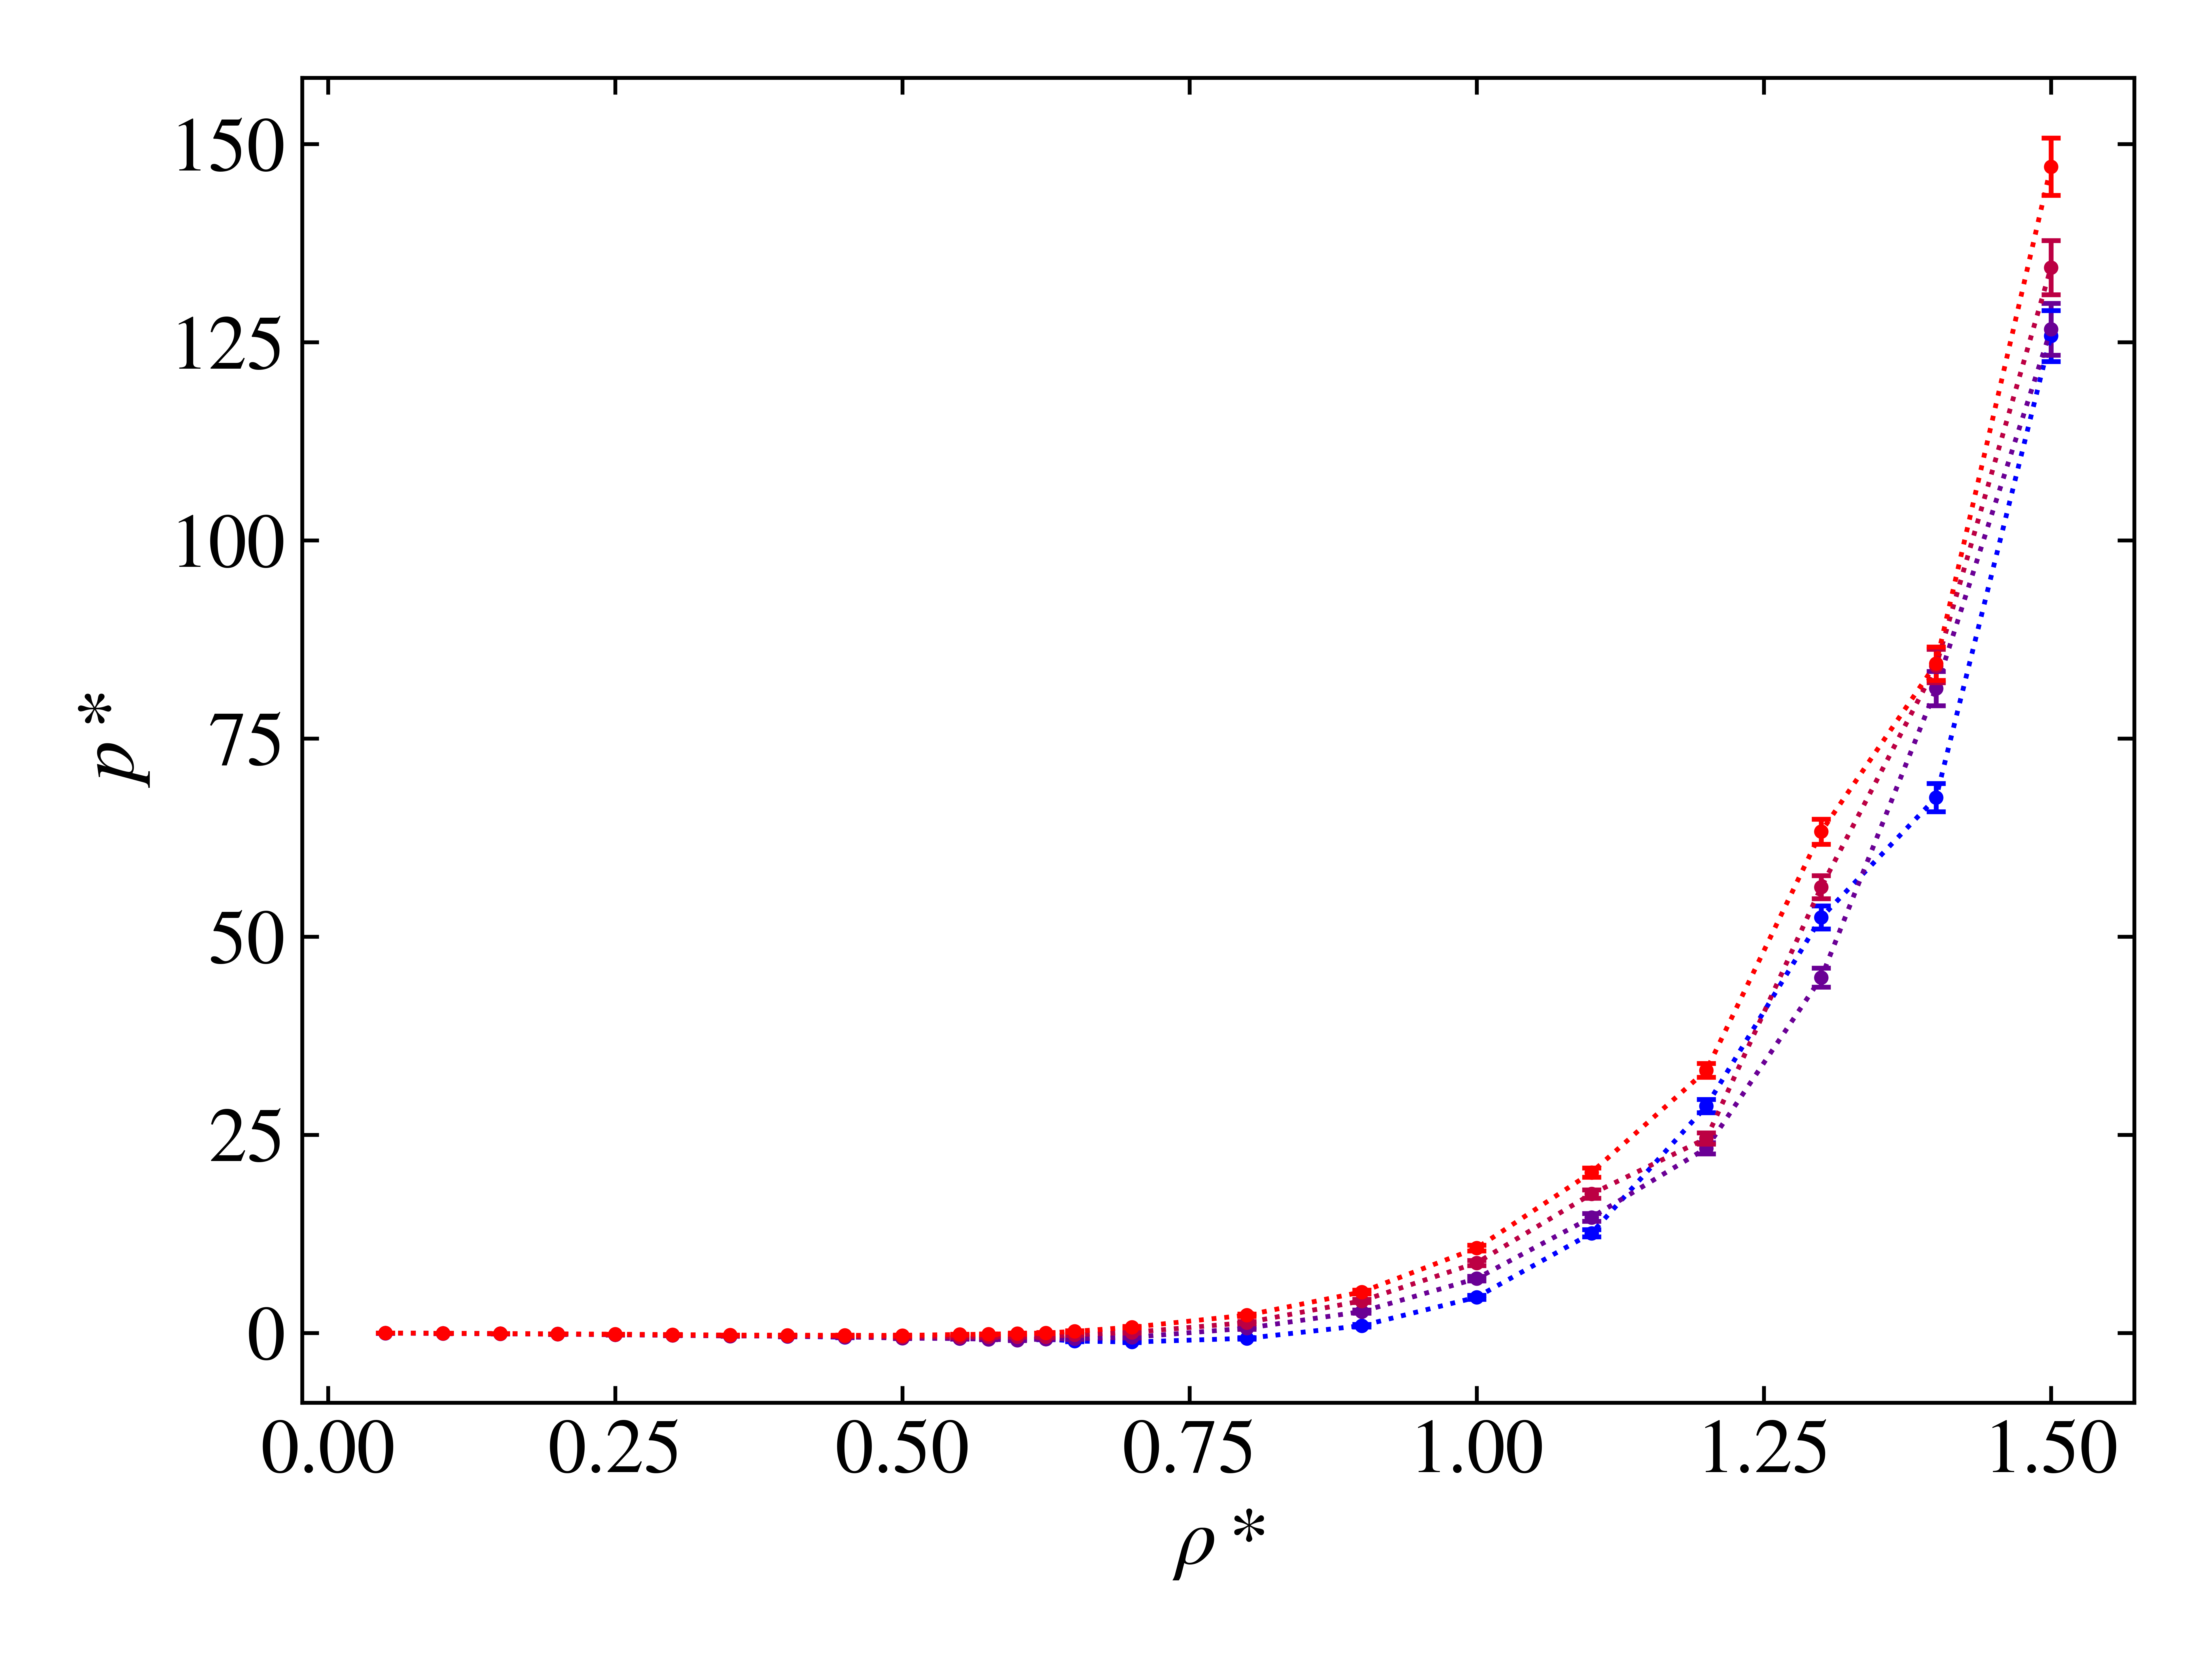
\includegraphics[width=\linewidth]{figures/excessEnergyPressure/excessPressure.png}
	\caption{MC results for the excess pressure, $p^{*}$, against density, $\rho{}^{*}$ along four isotherms $T^{*}=0.75, 1.00, 1.25, 1.50$, each represented by a colour ranging from blue to red. Error bars show the standard error in the mean. Dotted lines have been added to guide the eye.}
	\label{fig:excessPressure}
\end{figure}


\begin{figure}
	\includegraphics[width=\linewidth]{figures/rdfs/RDFs.png}
	\caption{Radial distribution functions (RDFs), $g(r^{*})$ of our MC systems along an isotherm $T^{*}=1.5$ at densities $\rho{}^{*}=0.1, 0.8, 1.5$ shown in the lower, middle, upper panel respectively. These typically correspond to vapour-like, liquid-like, solid-like states respectively. Markers are omitted for visual clarity.}
	\label{fig:RDFs}
\end{figure}

\begin{figure}
	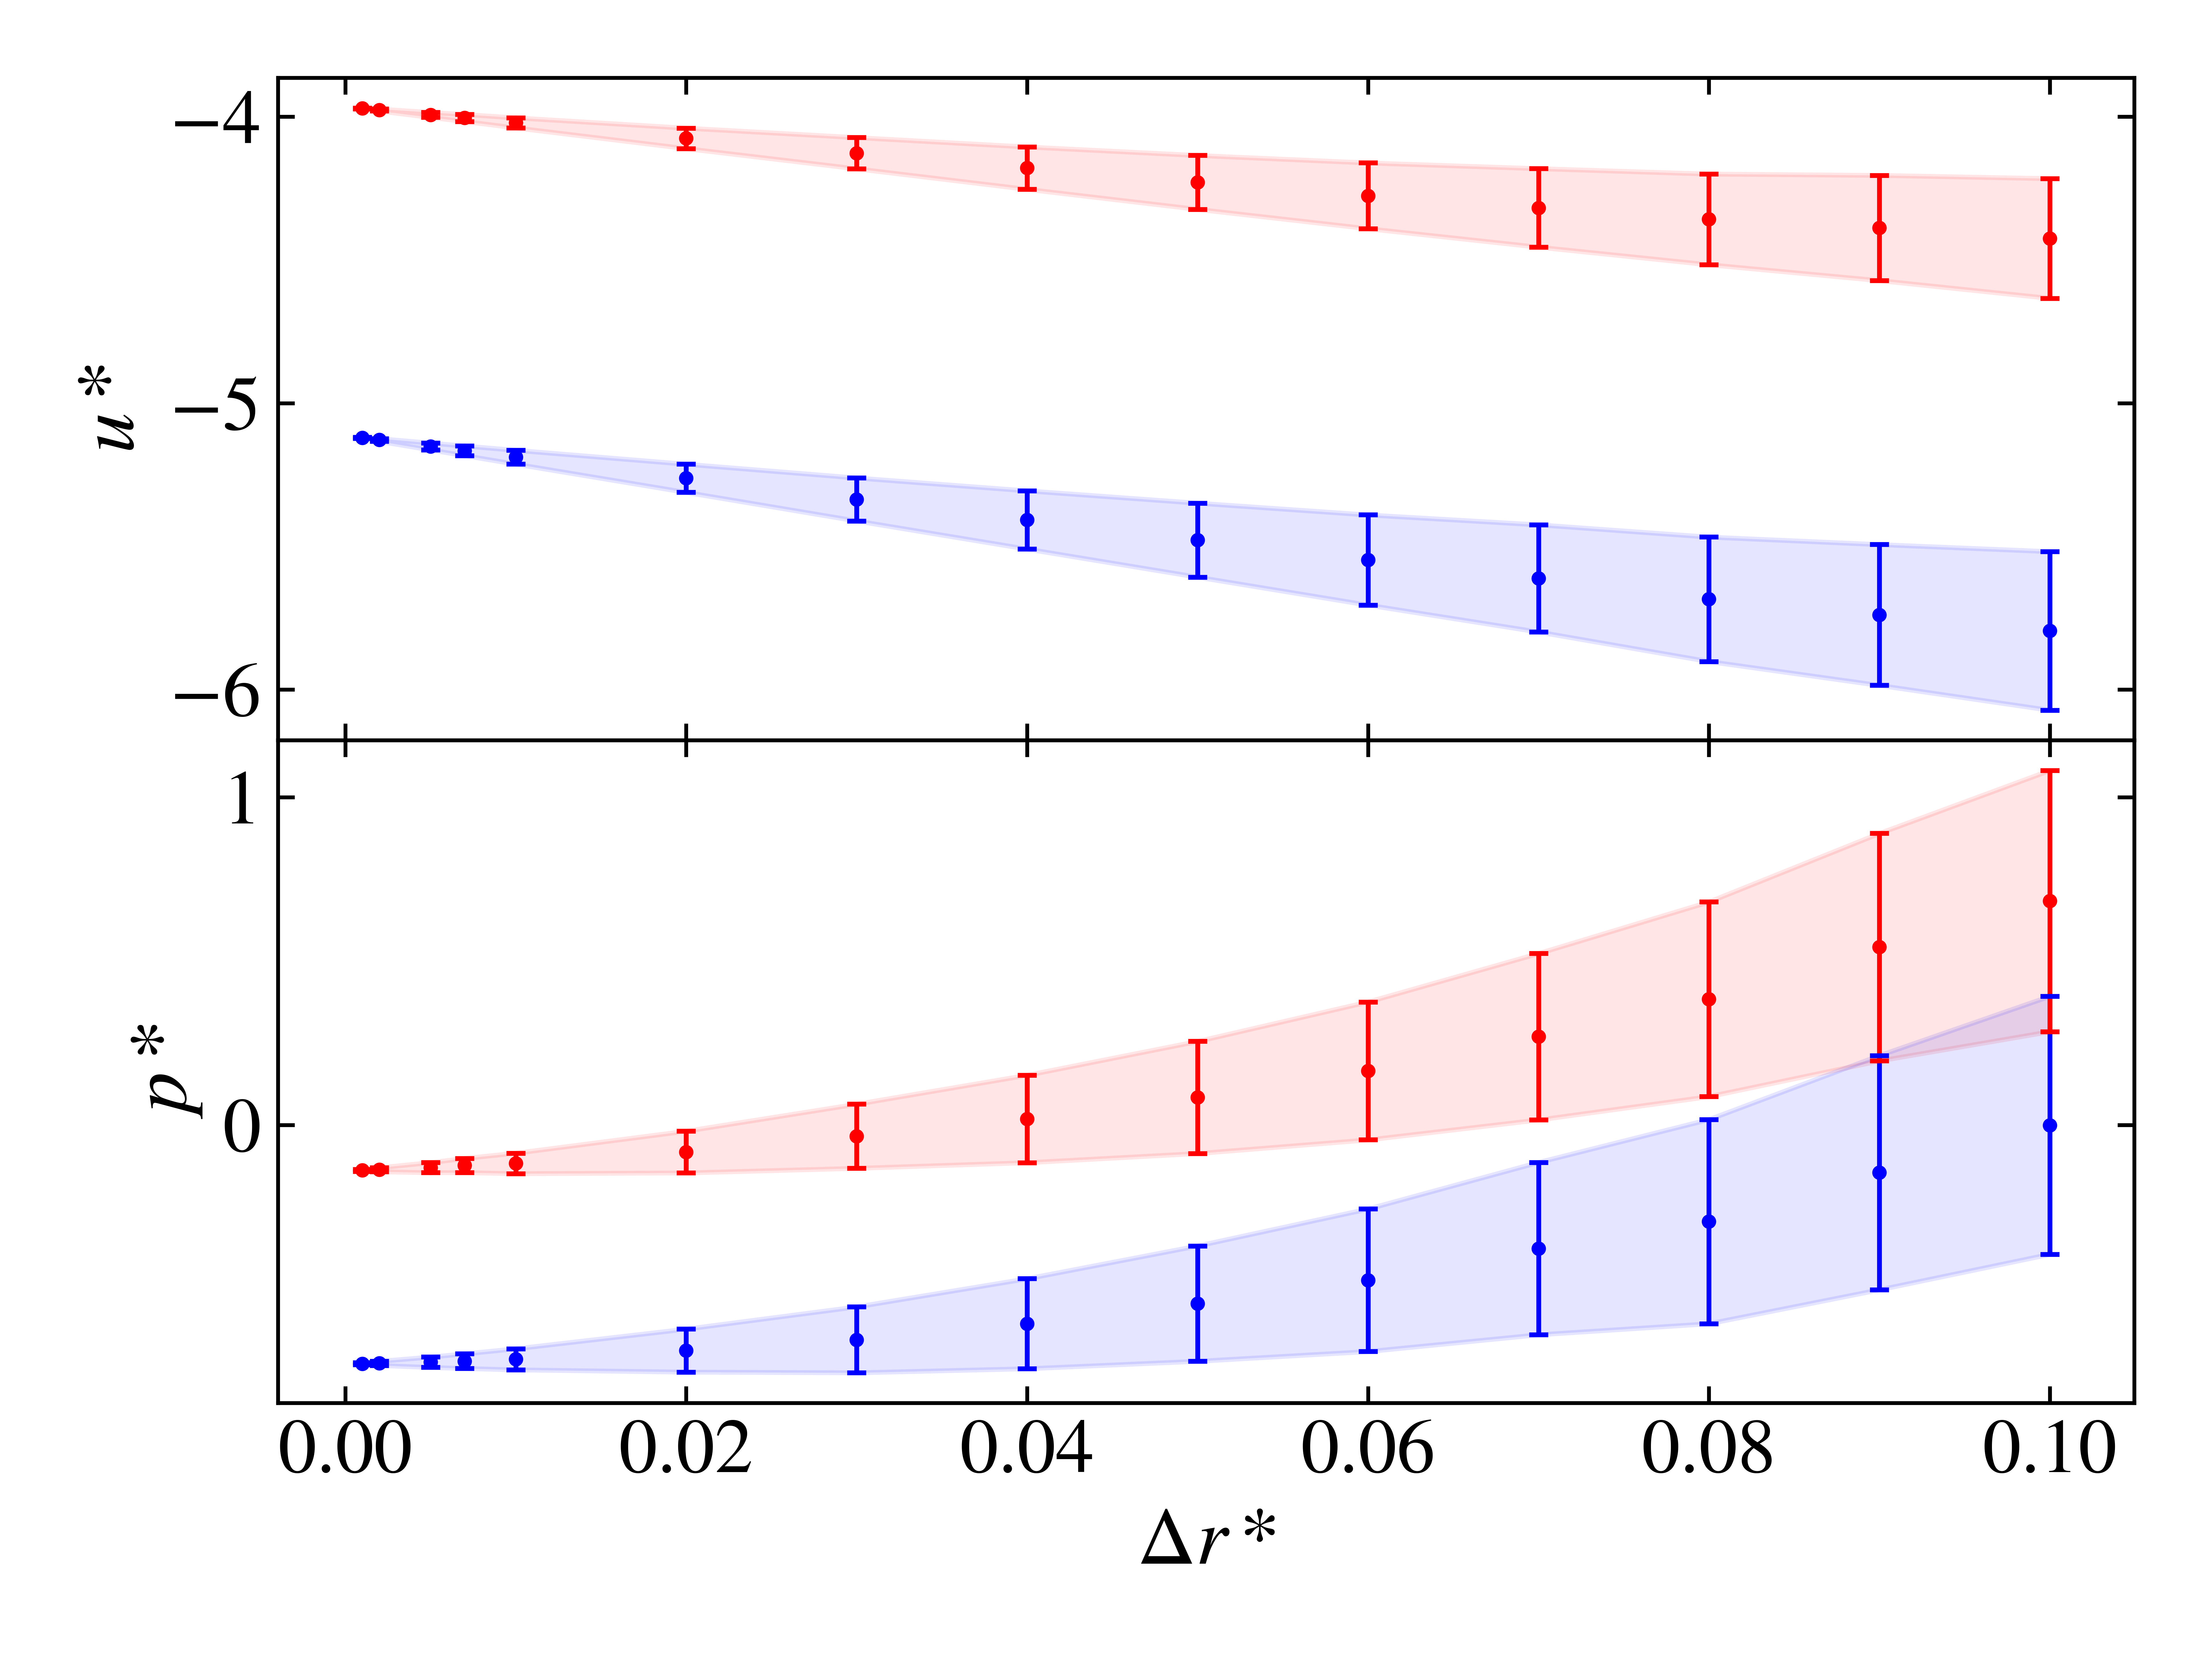
\includegraphics[width=\linewidth]{figures/binWidth/BWFeffect.png}
	\caption{Excess energy per particle, $u^{*}$, and excess pressure, $p^{*}$, against step-size $\Delta{}r^{*}$ (see discussion regarding equations \ref{eq:energy}, \ref{eq:pressure} in section \ref{s:methods}) evaluated for a system of density $\rho{}^{*}=0.6$ along isotherms $T^{*}=0.75, 1.5$ represented by blue and red markers respectively. Error bars show the standard error in the mean. Blue and red shaded areas are drawn to illustrate the increase in standard error with increasing step-size.}
	\label{fig:BWF}
\end{figure}

\begin{figure}
	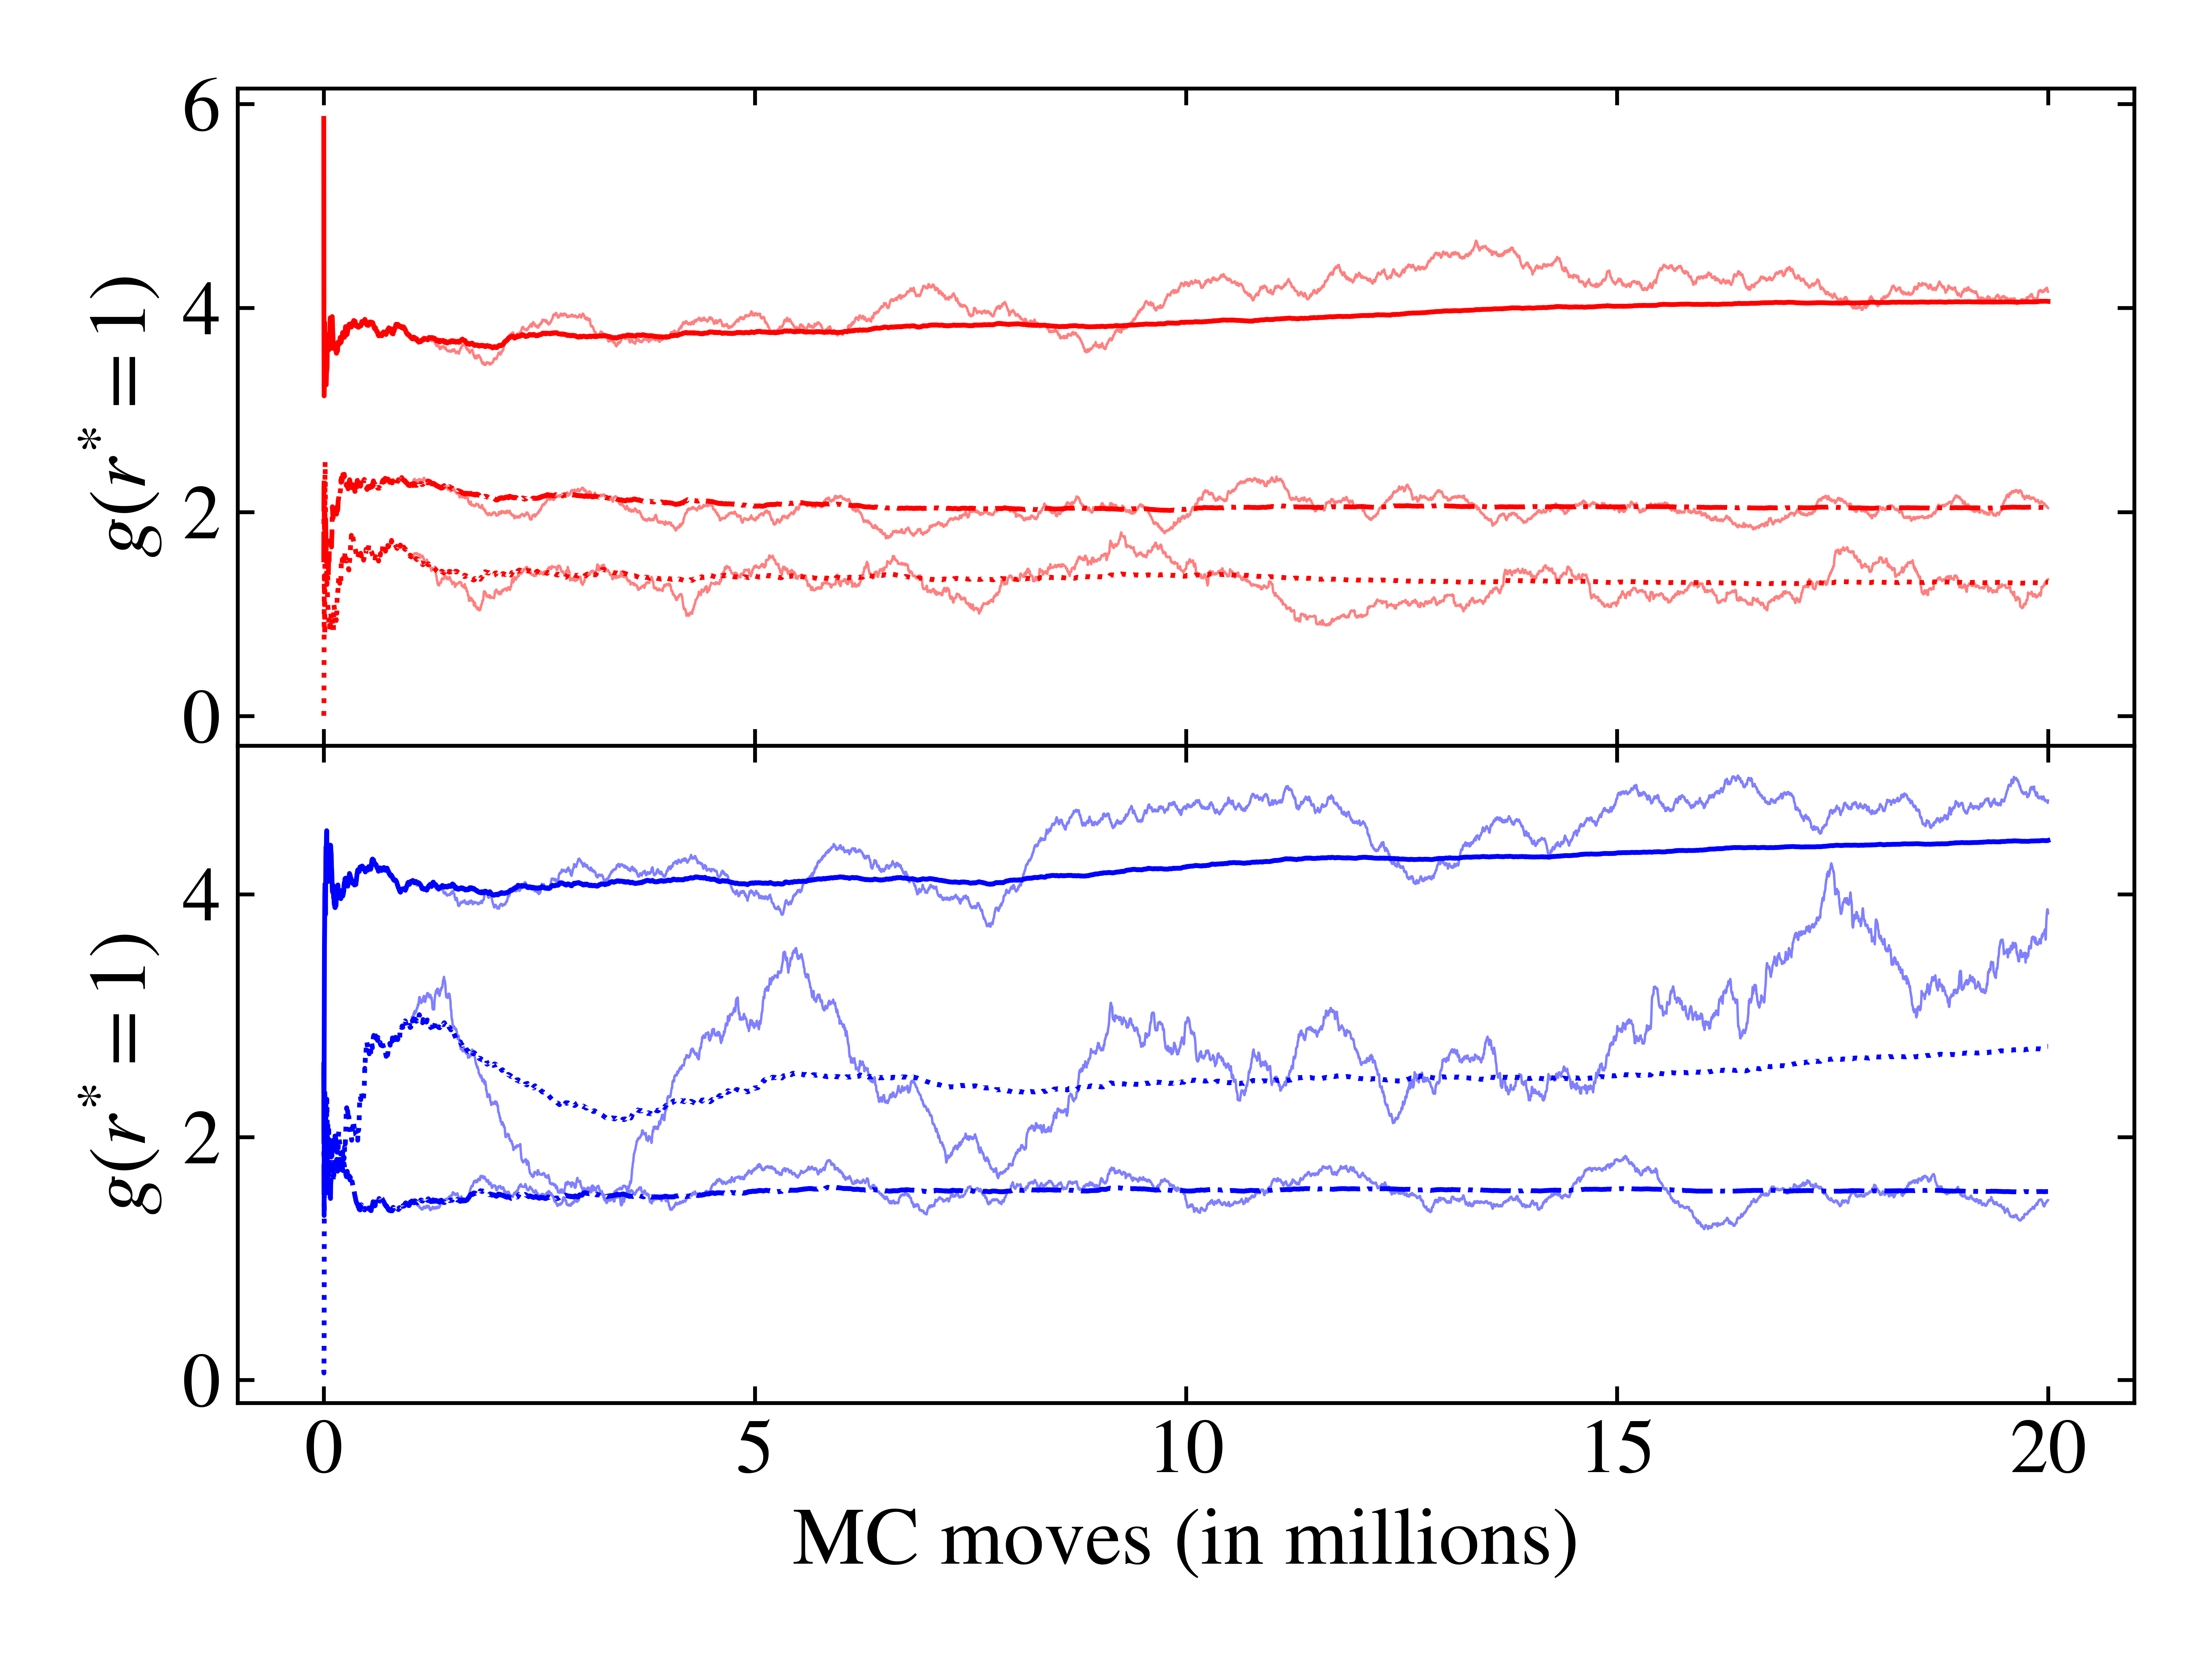
\includegraphics[width=\linewidth]{figures/convergence/gAtSigma_convergence.png}
	\caption{Typical convergence and fluctuation of the radial distribution function, $g(r^{*})$ evaluated at $r^{*}=1$. The smoother, darker lines show the variation of the cumulative average with increasing numbers of MC moves and are plotted for densities $\rho^{*} = 0.3, 0.8, 1.3$ represented by dotted, dash-dot, solid lines respectively. The lighter, jagged lines at any given point give a values of $g(r^{*}=1)$ averaged over the preceding 1 million MC moves. These are shown for isotherms $T^{*} = 0.75, 1.5$ represented by blue and red lines respectively. 
	}
	\label{fig:convergence}
\end{figure}

Typical radial distribution functions for the gaseous, liquid and crystalline solid states are presented in figure \ref{fig:RDFs}. [For each state we observe the RDF to be zero until almost $r^{*}=1$. This is due to the sharp increase in the LJ potential when $r^{*}<1$ and as such these are energetically unfavourable positions for particles to be in close to but less than $r^{*}=1$ and essentially prohibited at $r^{*}<<1$.] A sharp peak is observed at $r^{*}=1$ for each state, beyond which they become distinct. In the gaseous state, $g(r)$ quickly drops to unity beyond $r^{*}=1$, [indicating that the substance is entirely homogeneous and completely lacks order.] In the liquid state, $g(r)$ displays damped oscillatory behaviour beyond $r^{*}=1$, converging to $g(r)=1$ [shortly]. The oscillations in $g(r)$ indicate that at some points we are more or less likely to observe a particle at a given distance from a reference particle [but only up to some medium value beyond which the substance is homogeneous], i.e. short-range order is observed. In the crystalline solid state the formation of many irregular peaks and troughs in $g(r)$, indicating that we are very likely or unlikely to find particles in certain positions. This irregularity is observed over a longer distance than the oscillatory behaviour in the liquid state, indicating the presence of long-range order.


\section{Discussion} \label{s:analysis}
%\lipsum[1-15]


\section{Conclusions} \label{s:conclusions}
%\lipsum[1-5]

\begin{thebibliography}{}

\bibitem{ref01} A. N. Other, Title of the Book, edition, publishers, place of publication (year of publication), p. 123.   % example reference

\bibitem{errors}I. G. Hughes, T. P. A Hase, Measurements and their Uncertainties A Practical Guide to Modern Error Analysis, 1st, Oxford University Press, Oxford (2010)

\end{thebibliography} 

\clearpage
\appendix
\section{Error Analysis} \label{a:errors}
All propagation of errors is performed as outlined in \cite{errors}.

\clearpage
\section{Comparison to NIST data} \label{a:NIST}


% Please add the following required packages to your document preamble:
% \usepackage{booktabs}
% \usepackage{multirow}
% \usepackage{graphicx}
\begin{table}[]
	\resizebox{\textwidth}{!}{%
		\begin{tabular}{@{}rrrrrrrrrr@{}}
			\toprule
			$T^*$                  & $\rho{}^*$ & $U_\text{NIST}^*$ & $\pm$    & $U_\text{ours}^*$ & $\pm$   & $p_\text{NIST}^*$ & $\pm$    & $p_\text{ours}^*$ & $\pm$   \\ \midrule
			\multirow{10}{*}{0.85} & 1.00E-3    & -1.0317E-2       & 2.34E-5 & -9.968E-3         & 9.17E-5 & 8.4402E-4        & 4.66E-8 & -5.288E-6         & 1.72E-7 \\
			& 3.00E-3    & -3.1019E-2       & 5.91E-5 & -3.156E-2         & 2.87E-4 & 2.4965E-3        & 4.99E-7 & -6.121E-5         & 1.48E-6 \\
			& 5.00E-3   & -5.1901E-2       & 7.53E-5 & -5.485E-2         & 5 .07E-4 & 4.1003E-3        & 5.05E-7 & -1.472E-4         & 4.75E-6 \\
			& 7.00E-3   & -7.2834E-2       & 1.34E-4 & -7.499E-2         & 6.87E-4 & 5.6565E-3        & 7.96E-7 & -2.854E-4         & 8.98E-6 \\
			& 9.00E-3   & -9.3973E-2       & 1.29E-4 & -9.863E-2         & 9.18E-4 & 7.1641E-3        & 2.24E-6 & -4.568E-4         & 1.51E-5 \\
			& 7.76E-1   & -5.5121       & 4.55E-4 & -5.623            & 5.21E-2 & 6.7714E-3        & 1.77E-3 & -5.577E-1         & 9.91E-2 \\
			& 7.80E-1   & -5.5386       & 7.26E-4 & -5.611            & 5.14E-2 & 4.7924E-2        & 3.18E-3 & -6.311E-1         & 9.88E-2 \\
			& 8.20E-1   & -5.7947       & 6.03E-4 & -5.908            & 5.59E-2 & 5.5355E-1        & 4.13E-3 & 2.588E-1          & 1.25E-1 \\
			& 8.60E-1   & -6.0305       & 2.38E-3 & -6.175            & 5.87E-2 & 1.2660        & 1.36E-2 & 4.973E-1          & 1.41E-1 \\
			& 9.00E-1   & -6.2391       & 5.27E-3 & -6.346            & 6.17E-2 & 2.2314        & 2.72E-2 & 1.823             & 1.75E-1 \\ \cmidrule(lr){1-10}
			\multirow{10}{*}{0.90} & 1.00E-3   & -9.9165E-3       & 1.89E-5 & -9.989E-3         & 9.05E-5 & 8.9429E-4        & 2.48E-8 & -6.475E-6         & 1.76E-7 \\
			& 3.00E-3   & -2.9787E-2       & 3.21E-5 & -3.065E-2         & 2.79E-4 & 2.6485E-3        & 2.54E-7 & -4.368E-5         & 1.70E-6 \\
			& 5.00E-3   & -4.9771E-2       & 3.80E-5 & -5.226E-2         & 4.75E-4 & 4.3569E-3        & 2.19E-7 & -1.426E-4         & 4.35E-6 \\
			& 7.00E-3   & -6.9805E-2       & 7.66E-5 & 7.179E-2          & 6.50E-4 & 6.0193E-3        & 1.02E-6 & -3.075E-4         & 8.14E-6 \\
			& 9.00E-3   & -8.9936E-2       & 2.44E-5 & -9.151E-2         & 8.33E-4 & 7.6363E-3        & 1.44E-6 & -4.295E-4         & 1.41E-5 \\
			& 7.76E-1   & -5.4689       & 4.20E-4 & -5.615            & 5.21E-2 & 2.4056E-1        & 2.74E-3 & -2.486E-1         & 1.04E-1 \\
			& 7.80E-1   & -5.4956       & 7.86E-4 & -5.627            & 5.20E-2 & 2.7851E-1        & 2.97E-3 & -2.576E-1         & 1.06E-1 \\
			& 8.20E-1   & -5.7456       & 7.51E-4 & -5.870            & 5.53E-2 & 8.2386E-1        & 2.85E-3 & 2.921E-1          & 1.25E-1 \\
			& 8.60E-1   & -5.9753       & 5.53E-4 & -6.130            & 5.89E-2 & 1.5781        & 3.29E-3 & 1.193             & 1.53E-1 \\
			& 9.00E-1   & -6.1773       & 1.57E-3 & -6.312            & 6.14E-2 & 2.5848        & 9.54E-3 & 1.871             & 1.75E-1 \\ \bottomrule
		\end{tabular}%
	}
\end{table}

\end{document}